\documentclass[12pt, a4paper]{article}
\usepackage{../../../myconfig_line} % Gọi file cấu hình từ ngoài gốc vào
% ==========================================
% BẮT ĐẦU NỘI DUNG TÀI LIỆU
% ==========================================
\begin{document}

% Truyền 3 tham số: {Nhãn cam} {Chữ to chính giữa} {Chữ ở góc phải Header}
\titlebox{Chủ đề: Tích phân}{Ứng dung tích phân tính thể tích hình phẳng thực tế}{Nguyên hàm - Tích phân: Ứng dụng}


\questionTrueFalse{15}{1}{Một vật trang trí có dạng một khối tròn xoay được tạo thành khi quay miền \( (R) \) (phần gạch chéo trong hình vẽ) quanh trục \( MN \). Biết rằng \( ABCD \) là hình chữ nhật với \( AB = 6cm, AD = 10cm \) và \( M, N \) lần lượt là trung điểm của \( AB, CD \). Hai đường cong là đường Elip có hình chữ nhật cơ sở là \( ABCD \) và đường tròn tiếp xúc với hai cạnh \( AD \) và \( BC \) (tham khảo hình vẽ). Tính thể tích của vật trang trí đó ( kết quả làm tròn đến hàng chục theo đơn vị \(cm^3\)).
\begin{center}
\begin{tikzpicture}[scale=0.85, >=latex]

    % 1. Định nghĩa kích thước hình chữ nhật ABCD:
    % AB = 6cm -> nửa chiều cao b = 3
    % AD = 10cm -> nửa chiều rộng a = 5
    \pgfmathsetmacro{\a}{5}
    \pgfmathsetmacro{\b}{3}

    % Tọa độ 4 đỉnh hình chữ nhật
    \coordinate (A) at (-\a, \b);
    \coordinate (B) at (-\a, -\b);
    \coordinate (C) at (\a, -\b);
    \coordinate (D) at (\a, \b);

    % Trung điểm M của AB và N của CD
    \coordinate (M) at (-\a, 0);
    \coordinate (N) at (\a, 0);

    % 2. Tô miền gạch chéo (R):
    % Miền gạch chéo nằm bên trong Elip x^2/a^2 + y^2/b^2 <= 1
    % và bên ngoài đường tròn x^2 + y^2 <= b^2
    \begin{scope}
        % Cắt theo hình Elip lớn
        \clip (0,0) ellipse ({\a} and {\b});
        
        % Tô gạch chéo phần Elip
        \pattern[pattern=north east lines, pattern color=black] 
            (-\a, -\b) rectangle (\a, \b);
            
        % Đè phần hình tròn trắng lên để loại bỏ phần gạch chéo bên trong hình tròn
        \fill[white] (0,0) circle (\b);
    \end{scope}

    % 3. Vẽ lại đường viền các hình cho rõ nét

    % Đường tròn bán kính R = b = 3 (tiếp xúc với AD và BC)
    \draw[thick, black] (0,0) circle (\b);

    % Đường Elip có hình chữ nhật cơ sở là ABCD (bán trục lớn a = 5, bán trục nhỏ b = 3)
    \draw[thick, black] (0,0) ellipse ({\a} and {\b});

    % Hình chữ nhật ABCD
    \draw[very thick, black] (A) -- (B) -- (C) -- (D) -- cycle;

    % 4. Đánh dấu điểm nút và ghi nhãn các đỉnh
    \fill[black] (A) circle (1.8pt) node[above left, font=\bfseries\itshape] {$A$};
    \fill[black] (B) circle (1.8pt) node[below left, font=\bfseries\itshape] {$B$};
    \fill[black] (C) circle (1.8pt) node[below right, font=\bfseries\itshape] {$C$};
    \fill[black] (D) circle (1.8pt) node[above right, font=\bfseries\itshape] {$D$};
    \fill[black] (M) circle (1.8pt) node[left, font=\bfseries\itshape] {$M$};
    \fill[black] (N) circle (1.8pt) node[right, font=\bfseries\itshape] {$N$};

\end{tikzpicture}
\end{center}

}{
    \textbf{a)} & Elip có phương trình \(\dfrac{x^2}{25} + \dfrac{y^2}{9} = 1\).
    & \textcolor{amberorange}{$\bigcirc$} & \textcolor{amberorange}{$\bigcirc$} \\ \hline
    
    \textbf{b)} & Đường tròn có phương trình \((x-5)^2 + y^2 = 9\).
    & \textcolor{amberorange}{$\bigcirc$} & \textcolor{amberorange}{$\bigcirc$} \\ \hline
    
    \textbf{c)} & Thể tích vật trang trí được tính bởi công thức  
    \(V = \pi \displaystyle\int_{-3}^{0} \left[ \left(3\sqrt{1-\dfrac{y^2}{9}}\right)^2 - \left(5 - \sqrt{9-y^2}\right)^2 \right] dy\).
    & \textcolor{amberorange}{$\bigcirc$} & \textcolor{amberorange}{$\bigcirc$} \\ \hline
    
    \textbf{d)} & Thể tích của vật trang trí là \(340 \, cm^3\) (làm tròn đến hàng chục).
    & \textcolor{amberorange}{$\bigcirc$} & \textcolor{amberorange}{$\bigcirc$} \\
}



\questionShortAnswer{25}{2}{Nếu cắt chậu nước có hình dạng như hình bên bằng mặt phẳng song song và cách mặt đáy \( x \) (cm) \((0 \leq x \leq 16)\) thì mặt cắt là hình tròn có bán kính \( R = 10 + \sqrt{x} \) (cm). Tìm \( x \) (đơn vị cm, làm tròn kết quả đến hàng phần trăm) để dung tích nước trong chậu bằng \(\dfrac{1}{2}\) thể tích của chậu?

\begin{center}
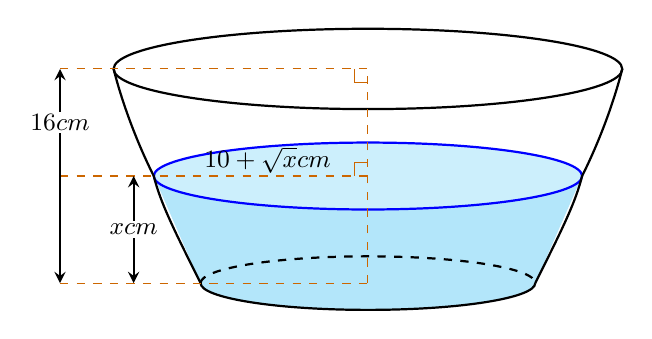
\begin{tikzpicture}[scale=0.85, >=latex]

    % 1. Định nghĩa các thông số hình học
    % Đáy chậu (x = 0): bán kính r_bottom = 2.5
    % Mặt nước (chiều cao x): h_water = 1.6, bán kính r_water = 3.2
    % Miệng chậu (chiều cao 16): h_top = 3.2, bán kính r_top = 3.8

    % 2. Tô màu khối nước (phần dưới của chậu)
    \fill[cyan!30] (-2.5, 0) arc (180:360:2.5cm and 0.4cm) 
        -- (3.2, 1.6) arc (0:180:3.2cm and 0.5cm) -- cycle;
    \fill[cyan!20] (0, 1.6) ellipse (3.2cm and 0.5cm);

    % 3. Vẽ thành chậu thủy tinh / gốm (phần trong suốt)
    % Đáy chậu
    \draw[thick, black] (-2.5, 0) arc (180:360:2.5cm and 0.4cm);
    \draw[dashed, thick, black] (-2.5, 0) arc (180:0:2.5cm and 0.4cm);

    % Mặt nước
    \draw[thick, blue] (0, 1.6) ellipse (3.2cm and 0.5cm);

    % Miệng chậu
    \draw[thick, black] (0, 3.2) ellipse (3.8cm and 0.6cm);

    % Đường cong thành chậu hai bên (mô phỏng hàm R = 10 + sqrt(x))
    \draw[thick, black] (-2.5, 0) .. controls (-2.9, 0.8) and (-3.1, 1.2) .. (-3.2, 1.6) 
                        .. controls (-3.5, 2.2) and (-3.7, 2.8) .. (-3.8, 3.2);
    \draw[thick, black] (2.5, 0) .. controls (2.9, 0.8) and (3.1, 1.2) .. (3.2, 1.6) 
                        .. controls (3.5, 2.2) and (3.7, 2.8) .. (3.8, 3.2);

    % 4. Các đường dóng kích thước màu cam (orange!80!black)
    % Đường dóng ngang đáy chậu, mặt nước và miệng chậu
    \draw[dashed, orange!80!black, thin] (-4.6, 0) -- (0, 0);
    \draw[dashed, orange!80!black, thin] (-4.6, 1.6) -- (0, 1.6);
    \draw[dashed, orange!80!black, thin] (-4.6, 3.2) -- (0, 3.2);

    % Đường dóng bán kính mặt nước (từ tâm ra mép)
    \draw[dashed, orange!80!black, thin] (0, 1.6) -- (0, 1.6);
    \draw[dashed, orange!80!black, thin] (0, 0) -- (0, 3.2);

    % Ký hiệu góc vuông
    \draw[orange!80!black, thin] (-0.2, 1.6) -- (-0.2, 1.8) -- (0, 1.8);
    \draw[orange!80!black, thin] (-0.2, 3.2) -- (-0.2, 3.0) -- (0, 3.0);

    % 5. Mũi tên và nhãn kích thước
    % Chiều cao tổng 16 cm (bên trái ngoài cùng)
    \draw[<->, >=stealth, thick, black] (-4.6, 0) -- (-4.6, 3.2);
    \node[fill=white, inner sep=1pt] at (-4.6, 2.4) {\small $16\text{ cm}$};

    % Chiều cao mực nước x cm (bên trái)
    \draw[<->, >=stealth, thick, black] (-3.5, 0) -- (-3.5, 1.6);
    \node[fill=white, inner sep=1pt] at (-3.5, 0.8) {\small $x\text{ cm}$};

    % Bán kính R = 10 + sqrt(x) cm trên mặt nước
    \node[above] at (-1.5, 1.5) {\small $10+\sqrt{x}\text{ cm}$};

\end{tikzpicture}
\end{center}
}


\questionShortAnswer{25}{3}{Một chậu cây có chiều cao 50cm và đường kính miệng chậu là 50cm. Mặt cắt ngang của chậu cây là một đường parabol (tham khảo hình vẽ).
\begin{figure}[htbp]
    \centering
    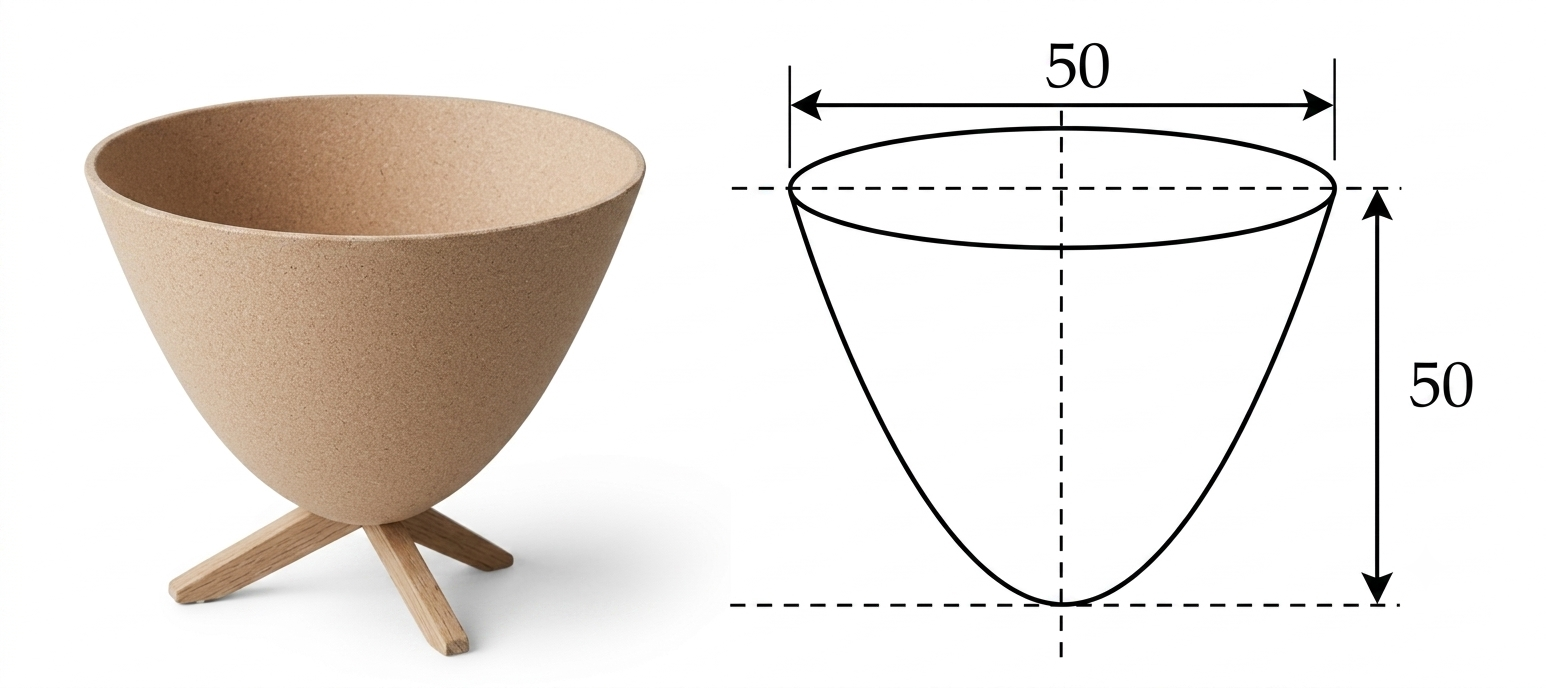
\includegraphics[width=0.5\textwidth]{../images/Chau.png}
\end{figure}

Tính thể tích của chậu cây đó (đơn vị dm\(^3\), kết quả làm tròn đến hàng phần chục).

}

\questionShortAnswer{23}{4}{Săm lớp xe ô tô khi bơm căng đặt nằm trên mặt phẳng nằm ngang có hình chiếu bằng như hình vẽ với bán kính đường tròn nhỏ \( R_1 = 25cm \), bán kính đường tròn lớn \( R_2 = 35cm \) và mặt cắt khi cắt bởi mặt phẳng đi qua trục, vuông góc với mặt phẳng nằm ngang là hai đường tròn. Bỏ qua độ dày của vỏ săm. Tính thể tích không khí được chứa bên trong săm, kết quả làm tròn đến hàng đơn vị của decimet khối.

\begin{center}
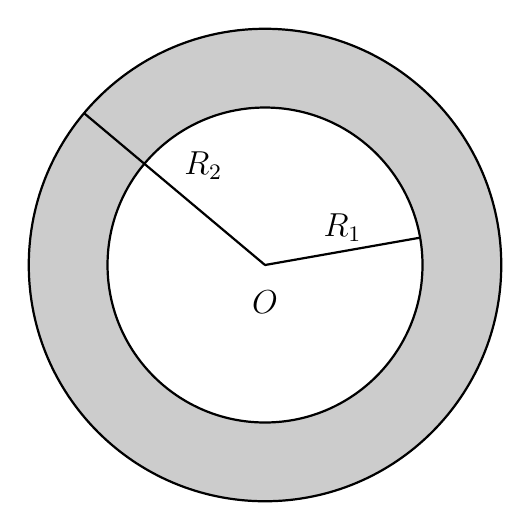
\begin{tikzpicture}[scale=0.1, >=latex]

    % 1. Định nghĩa bán kính trên hình
    % R1 = 20 (tương ứng 25 cm)
    % R2 = 30 (tương ứng 35 cm)
    
    % 2. Tô màu xám miền vành khăn giữa hai đường tròn
    \fill[gray!40, even odd rule] (0, 0) circle (30) (0, 0) circle (20);

    % 3. Vẽ hai đường tròn đồng tâm
    \draw[thick, black] (0, 0) circle (30);
    \draw[thick, black] (0, 0) circle (20);

    % 4. Vẽ các bán kính R1 và R2
    % Bán kính R1 (hướng góc ~ 10 độ)
    \draw[thick, black] (0, 0) -- (10:20);
    \node[above, font=\large] at (10:10) {$R_1$};

    % Bán kính R2 (hướng góc ~ 140 độ)
    \draw[thick, black] (0, 0) -- (140:30);
    \node[above right, font=\large] at (140:15) {$R_2$};

    % 5. Đánh dấu tâm O
    \fill[black] (0, 0) circle (3pt);
    \node[below, font=\large\itshape] at (0, -2) {$O$};

\end{tikzpicture}
\end{center}
}

\end{document}